\chapter{Server}
\section{Datenbank}
Die Verwendung einer Datenbank birgt große Vorteile. Insbesondere Skalierbarkeit und Erweiterbarkeit werden gesteigert. Zwar ist der Aufwand zunächst relativ hoch, macht sich auf lange Sicht jedoch positiv bemerkbar. Da Benutzerinformationen, Nachrichten etc dauerhaft gespeichert werden müssen, ist es ohnehin kaum möglich auf eine Datenbank zu verzichten. 
Die Wahl fiel auf MySQL da die Unterstützung für Java hervorragend ist und die Nutzung kostenlos ist. Des weiteren ist MySQL gut dokumentiert. Dank der MySQL Workbench ist es auch komfortabel die Datenbank zu warten und Einträge für Testzwecke zu erstellen.
Der Server verwendet Java Database Connectivity (JDBC) um mit der Datenbank zu kommunizieren. Mit Hilfe dieses Treibers ist es kein Problem Daten in der Datenbank zu speichern oder abzurufen.
Zu den Aufgaben der Datenbank gehört das Speichern der Nutzernamen samt Passwort hash welches für den Login benötigt wird. Darüber hinaus läuft das Nachrichtensystem über den Server. Nachrichten und Freundesliste werden von der Datenbank gespeichert. Die vorhandenen Spiele werden ebenfalls in der Datenbank abgelegt sowie die POI's.

\section{Webservices}
Wir verwenden RESTful Webservices. Auf Grund der Einschränkungen auf Seiten der App im Volley-Framework werden nur GET-Methoden verwendet. 

Bei allen Webservices außer der Registrierung wird das bei der Anmeldung enthaltene Token benötigt. Ist das mitgesendete Token nicht korrekt wird die Funktion verweigert.

\section{Benutzerverwaltung}
Sowohl die Registrierung neuer Benutzer als auch die Anmeldung bereits vorhandener Benutzer geht über den Server. 

\subsection{Registrierung}
Bei der Registrierung sendet der Benutzer seinen gewünschten Benutzernamen und den SHA-1 Hash seines Passwortes. Sofern der Benutzer noch nicht vorhanden ist wird dieser dann angelegt. Der Benutzer kann sich nun mit seinem Passwort anmelden.

\subsection{Anmeldung}
Die Anmeldung verläuft analog zur Registrierung. Auch hier wird der Benutzernamen und der SHA-1 Hash des Passwortes geschickt. Sind die Anmeldedaten korrekt(also in der Datenbank vorhanden), so wird ein Token für den Benutzer generiert und zurück gesendet.

\section{Tokenverwaltung}
Ohne ein gültiges Token kann ein Benutzer keine Aktionen ausführen. Ein Token verfällt nach einer gewissen Zeit der Inaktivität. Bei jeder Aktion eines Benutzers wird die Haltbarkeit des Tokens wieder erneuert. Ist das Token abgelaufen, so muss sich der Benutzer erneut anmelden.

Zusätzlich zu der Prüfung bei Aktionen von Benutzern werden Tokens regelmäßig auf ihre Gültigkeit getestet. Dies wird gemacht um zu verhindern, dass sich verfallene Tokens anhäufen.

\section{Minispiele}
Allgemein gilt, dass die gesamte Logik aller Spiele auf dem Server abläuft. Lediglich die Darstellung der Spiele wird in der App geregelt.

\subsection{Factory}
Für die Minispiele verwenden wir eine abstrakte Basisklasse, die alle Daten beinhaltet, die für jedes Spiel relevant sind, unabhängig das Typs. Die Klasse selbst erweitert \lstinjava{Thread}.

Die Spiele werden über eine Factory erzeugt. Diese erzeugt nicht nur die Spiele sondern verwaltet auch die Spielinstanzen und die Wartelisten der Spieler. 

\subsection{Warteschlange}
Wenn ein Spieler sich für ein Spiel anmeldet kommt er in die Warteschlange für dieses Spiel. Sobald genügend Spieler für das Spiel vorhanden sind wird die Spielinstanz erzeugt.

\subsection{Instantiierung}
Bei der Instantiierung wird eine neue Instanz des Spiels erzeugt. Anschließend werden die Spieler dem Spiel zugewiesen. Sobald alle Spieler bereit sind wird das Spiel gestartet.

\subsection{Rock, Paper, Scissors, Lizzard, Spock}
Rock, Paper, Scissors, Lizzard, Spock ist eine abgewandelte Version von Stein, Schere, Papier. Diese ist bekannt aus \textit{The Big Bang Theory}. 

\subsubsection{Regeln}
Die Regeln basieren auf denen von Stein, Schere, Papier. In der Abbildung sind die Regeln dargestellt.

\begin{capfigure}[Rock, Paper, Scissors, Lizzard, Spock Regeln]
	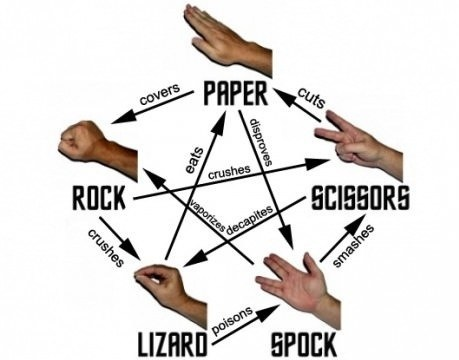
\includegraphics[width=10cm]{images/rpssl_rules}
\end{capfigure}

Für die Umsetzung der Regeln wurde eine Klasse \lstinjava{GameRule} verwendet. Zudem gibt es noch die Klasse \lstinjava{GameHand}, die die einzelnen Hände abbildet. In der Klasse \lstinjava{GameRule} gibt es immer eine erste Hand, eine zweite Hand und ein Ergebnis. Die möglichen Kombinationen werden in einer Liste gespeichert.

\section{Übertragung der Chatnachrichten}
Für die Übertragung der Chatnachrichten gibt es zwei Funktionen. Eine Funktion zum Senden neuer Nachrichten und eine Funktion zum Abfragen der Nachrichten.

Beim Abfragen der Nachrichten wird neben dem Token der eigene Benutzername, so wie der Benutzername des Chatpartners an die Anfrage angefügt. Als Ergebnis liefert der Server eine Liste der Chatnachrichten zwischen den beiden Teilnehmern. Die Liste wird beim  als JSON-String gesendet.

Beim Senden einer neuen Chatnachricht wird neben dem Token die Chatnachricht als JSON-String übertragen. Da ein JSON-String Zeichen enthält, die bei URLs nicht erlaubt sind und daher mit einer GET-Methode nicht funktionieren würde, wird der JSON-String vor dem Senden noch in seine Hexadezimal-Darstellung umgewandelt.